%% LaTeX-Beamer template for KIT design
%% by Erik Burger, Christian Hammer
%% title picture by Klaus Krogmann
%%
%% version 2.1
%%
%% mostly compatible to KIT corporate design v2.0
%% http://intranet.kit.edu/gestaltungsrichtlinien.php
%%
%% Problems, bugs and comments to
%% burger@kit.edu

\documentclass[18pt]{beamer}

%% SLIDE FORMAT

% use 'beamerthemekit' for standard 4:3 ratio
% for widescreen slides (16:9), use 'beamerthemekitwide'
\usepackage[utf8]{inputenc}
\usepackage[T1]{fontenc}
\usepackage{templates/beamerthemekit}
\usepackage{templates/tikzkit}
% \usepackage{templates/beamerthemekitwide}

%% TITLE PICTURE

% if a custom picture is to be used on the title page, copy it into the 'logos'
% directory, in the line below, replace 'mypicture' with the 
% filename (without extension) and uncomment the following line
% (picture proportions: 63 : 20 for standard, 169 : 40 for wide
% *.eps format if you use latex+dvips+ps2pdf, 
% *.jpg/*.png/*.pdf if you use pdflatex)

%\titleimage{mypicture}

%% TITLE LOGO

% for a custom logo on the front page, copy your file into the 'logos'
% directory, insert the filename in the line below and uncomment it

\titlelogo{ElipseLogo}

% (*.eps format if you use latex+dvips+ps2pdf,
% *.jpg/*.png/*.pdf if you use pdflatex)

%% TikZ INTEGRATION

% use these packages for PCM symbols and UML classes
% \usepackage{templates/tikzkit}
% \usepackage{templates/tikzuml}

% the presentation starts here

\title[Elipse]{Elipse -- Einteilungs Interface für das PSE}
\subtitle{Abschlusspräsentation}
\author{D. Biester, E. Dohse, P. Faller, P. Loth, L. Seufert, S. Kopmann}
\institute{IPD Snelting}

% Bibliography

\usepackage[citestyle=authoryear,bibstyle=numeric,hyperref,backend=biber]{biblatex}
\addbibresource{templates/example.bib}
\bibhang1em

\begin{document}

% change the following line to "ngerman" for German style date and logos
\selectlanguage{ngerman}

%title page
\begin{frame}
\titlepage
\end{frame}

%table of contents
% \begin{frame}{Gliederung}
% \tableofcontents
% \end{frame}

\section{Motivation}
\begin{frame}{Motivation des Projektes}
\begin{itemize}
\item Administrativen Aufwand minimieren
\item Speziell auf PSE zugeschnitten
\item Verbesserung gegenüber bestehender Systeme
\item Gute Ergebnisse für Studenten

\end{itemize}
\end{frame}

% \section{Ziele}
% \begin{frame}{Ziele}
% \begin{itemize}
% \item Geringere Änderungen an Studentensicht
% \item Komplette Verwaltung über ein Webinterinface
% \item Zusätzlicher Zugriff für Betreuer
% \item Bei Webinscribe fehlende Funktionen hinzufügen
% \item Erweiterbarkeit gewährleisten
% \item Berechnungszeit reduzieren
% \end{itemize}
% \end{frame}
\section{Live-Demo}
\begin{frame}
 \begin{center}
  \Huge Live-Demo
 \end{center}
\end{frame}
\section{Statistiken}
\subsection{LOC}
% Zahlen durch Diagramm ersetzen
\begin{frame}{Statistiken}
	\begin{tikzpicture}
		\draw[fill=kit-green70, thick] (0,0) -- (0:3cm) arc (0:163:3cm)
		node at (90:1.5cm) {45 \%};
		\draw (23:3cm) -- (23:3.5cm) node[right] {Programmcode, 7\,387 LOC};
		
		\draw[fill=kit-blue30!70!blue, thick] (0,0) -- (163:3cm) arc (163:360:3cm)
		node at (270:1.5cm) {55 \%};
		\draw (337:3cm) -- (337:3.5cm) node[right] {Testcode, 8\,890 LOC};
	\end{tikzpicture}
		
	\begin{itemize}
		\item Insgesamt 16\,277 Lines of Code
	\end{itemize}
\end{frame}
	%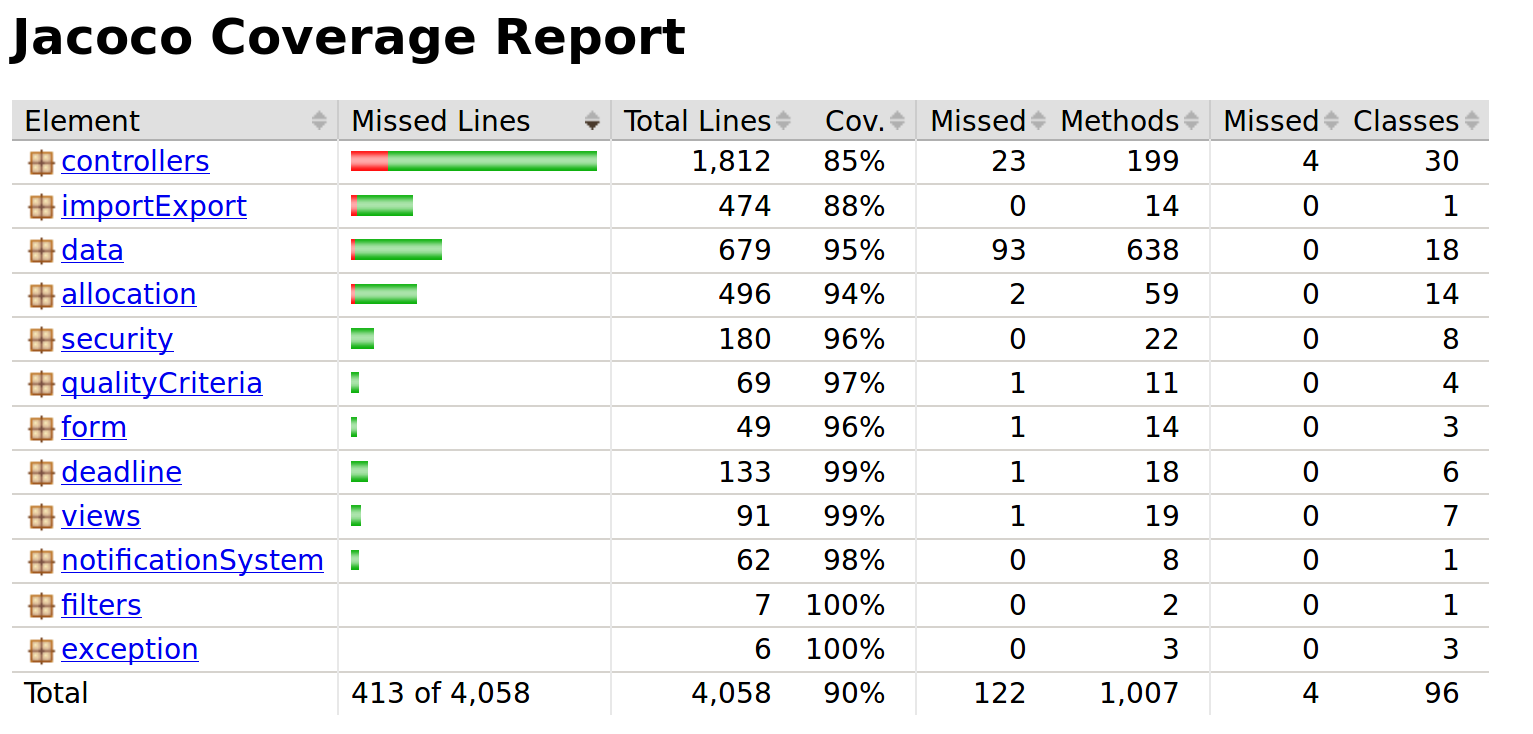
\includegraphics[width=\linewidth]{bilder/jacoco.png}
\subsection{Testabdeckung}	
\begin{frame}
	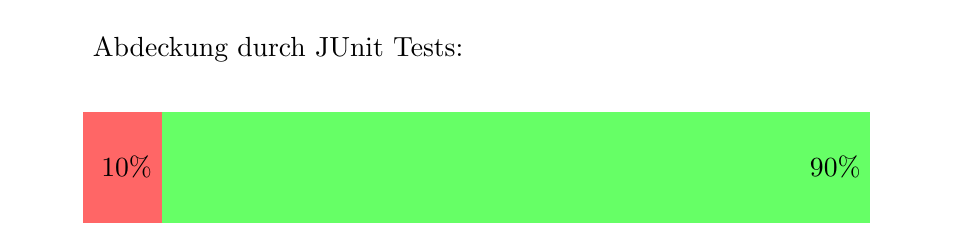
\begin{tikzpicture}[x={(0.1,0)},y={(0,0.1)}]
		\draw (0,15) node[right]{
			Abdeckung durch JUnit Tests:
		};
		%\draw[xshift=-4] (0,20) node[left]{Abgedeckt} (0, 0) node[left]{Nicht abgedeckt};
		\draw[line width=40,green!60] (10,0) plot [xcomb]
		coordinates {(100,0)};
		\draw[line width=40,red!60] (0,0) plot [xcomb]
		coordinates {(10,0)};
		\draw(100,0) node[left]{90\%} (10, 0) node[left]{10\%};
		
	\end{tikzpicture}
\end{frame}

\section{Bibliotheken}
\subsection{Bibliotheken}
% Folie mit verwendeten Tools
\begin{frame}{Verwendete Bibliotheken}
	\begin{tabular}{ccc}
		
\includegraphics[width=0.3\linewidth, height=0.3\textheight, keepaspectratio]{bilder/play_full_color.png} &
		
\includegraphics[width=0.3\linewidth, height=0.3\textheight, keepaspectratio]{bilder/ebean.png} &
		
\includegraphics[width=0.3\linewidth, height=0.3\textheight, keepaspectratio]{bilder/gurobi.png}\\
		%
\includegraphics[width=0.3\linewidth, height=0.3\textheight, keepaspectratio]{bilder/mysql.png} &
		
\includegraphics[width=0.3\linewidth, height=0.3\textheight, keepaspectratio]{bilder/pac4j.png}&
		
\includegraphics[width=0.3\linewidth, height=0.3\textheight, keepaspectratio]{bilder/apache.png}&
		
\includegraphics[width=0.3\linewidth, height=0.3\textheight, keepaspectratio]{bilder/keyczar.jpg} \\
	\end{tabular}
\end{frame}

\subsection{Werkzeuge}
\begin{frame}{Verwendete Werkzeuge}
	\begin{tabular}{ccc}
		
\includegraphics[width=0.3\linewidth, height=0.3\textheight, keepaspectratio]{bilder/eclipse.png} &
		
\includegraphics[width=0.3\linewidth, height=0.3\textheight, keepaspectratio]{bilder/papyrus.png} &
		
\includegraphics[width=0.3\linewidth, height=0.3\textheight, keepaspectratio]{bilder/github.png}\\
		
\includegraphics[width=0.3\linewidth, height=0.3\textheight, keepaspectratio]{bilder/junit.png} &
		
\includegraphics[width=0.3\linewidth, height=0.3\textheight, keepaspectratio]{bilder/mockito.png} &
		
\includegraphics[width=0.3\linewidth, height=0.3\textheight, keepaspectratio]{bilder/jacoco_logo.png} \\
		
\includegraphics[width=0.3\linewidth, height=0.3\textheight, keepaspectratio]{bilder/sonarqube.png}&
		%Plz don't hate. Ich weiß, dass es \LaTeX gibt. So war unkomplizierter.
		
\includegraphics[width=0.3\linewidth, height=0.3\textheight, keepaspectratio]{bilder/latex.png}&
		%
\includegraphics[width=0.3\linewidth, height=0.3\textheight, keepaspectratio]{bilder/keyczar.jpg}
		\\
	\end{tabular}
	
\end{frame}

\section{Reflexion}
\subsection{Schwierigkeiten}
\begin{frame}{Schwierigkeiten während des Projektes}
\only<+>{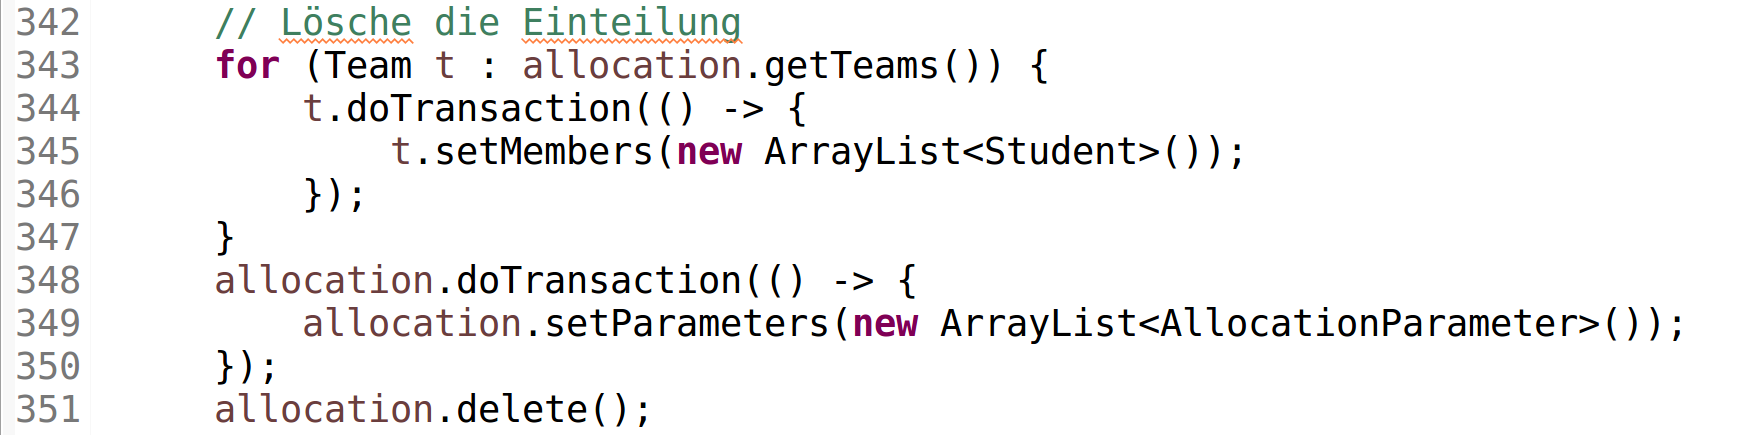
\includegraphics[trim = 0 0 0 390pt, clip, width=\linewidth]{bilder/ebeanScreenshot.png}}
\only<+>{\centering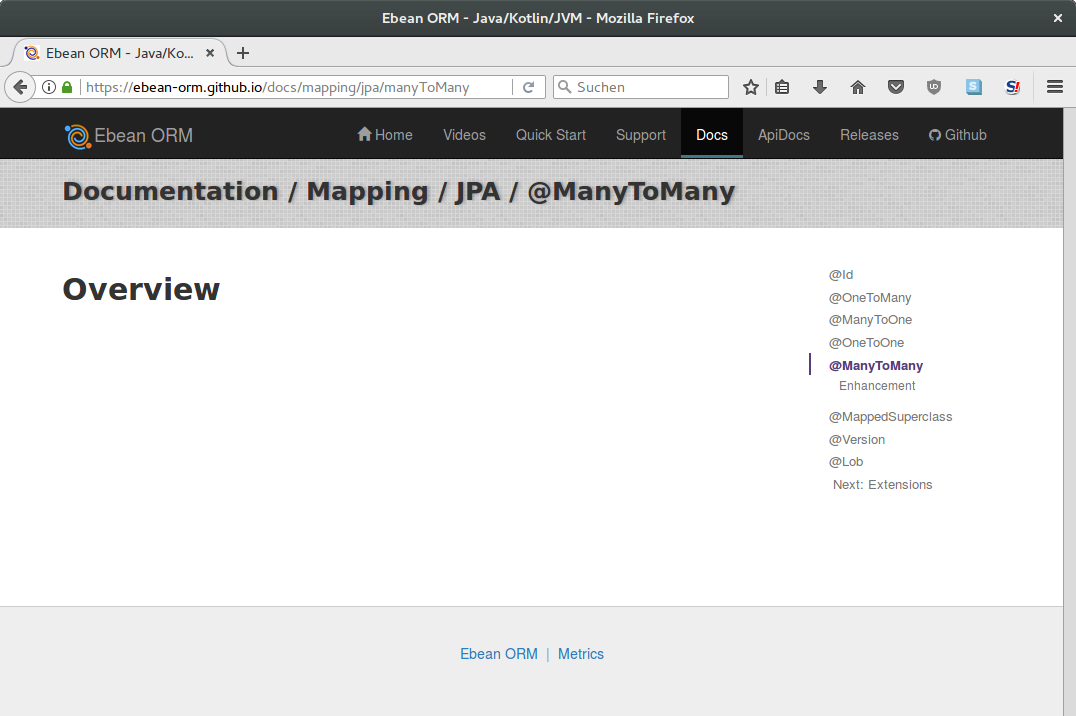
\includegraphics[width=0.9\linewidth]{bilder/ebeanDokuScreenshot.png}}
\only<+>{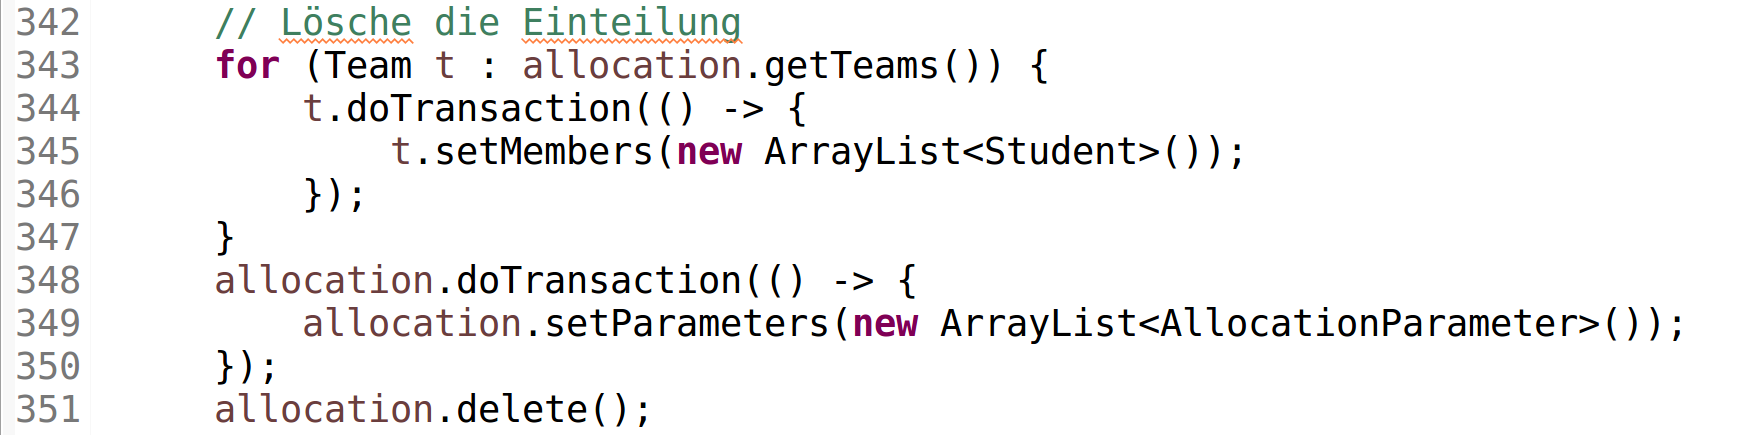
\includegraphics[width=\linewidth]{bilder/ebeanScreenshot.png}}
\end{frame}


\subsection{Ergebnis}
\begin{frame}{Ergebnis} 
\only<+>{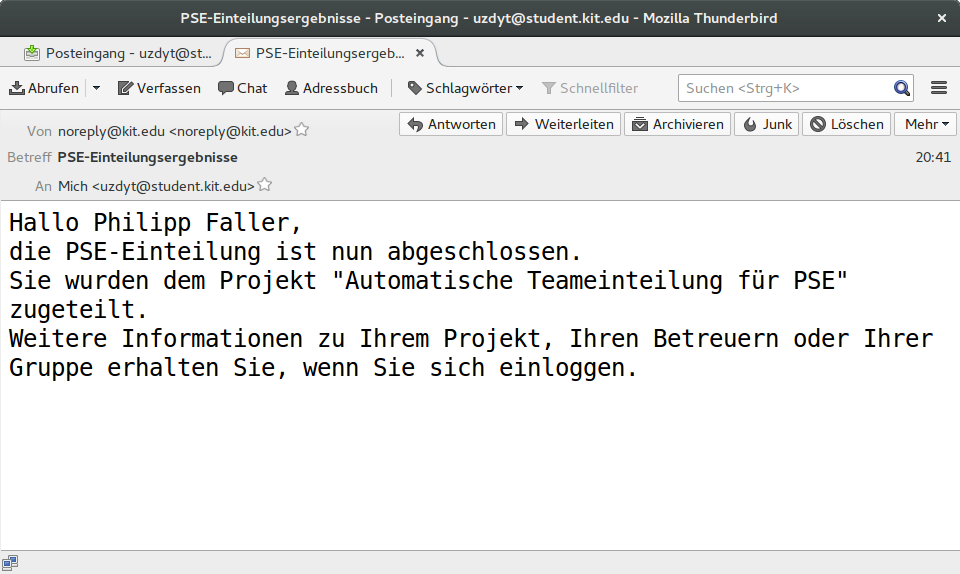
\includegraphics[width=\linewidth]{bilder/emailScreenshot.png}}
\only<+>{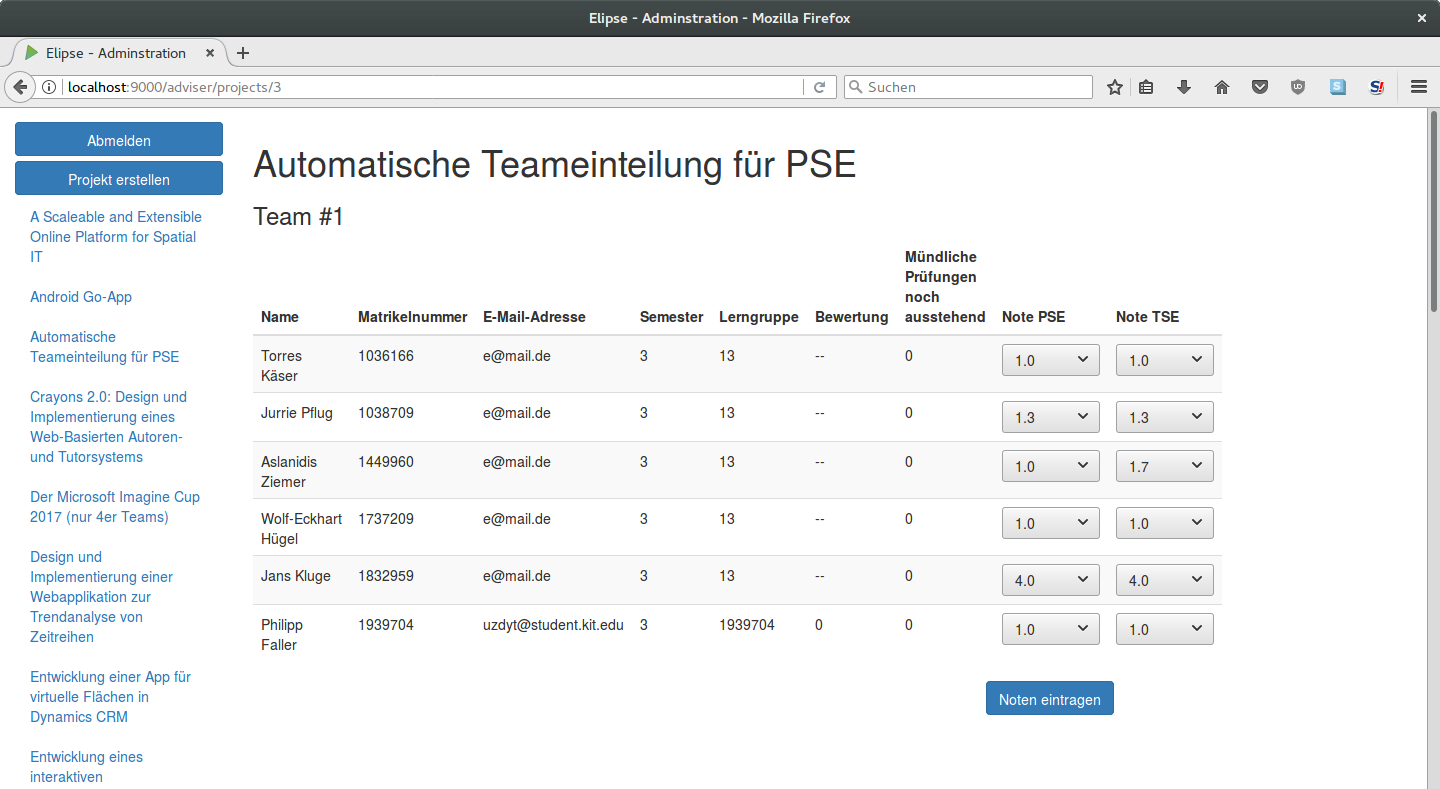
\includegraphics[width=\linewidth]{bilder/betreuerScreenshot.png}}
\only<+>{\centering{
	\begin{tabular}{lr}
	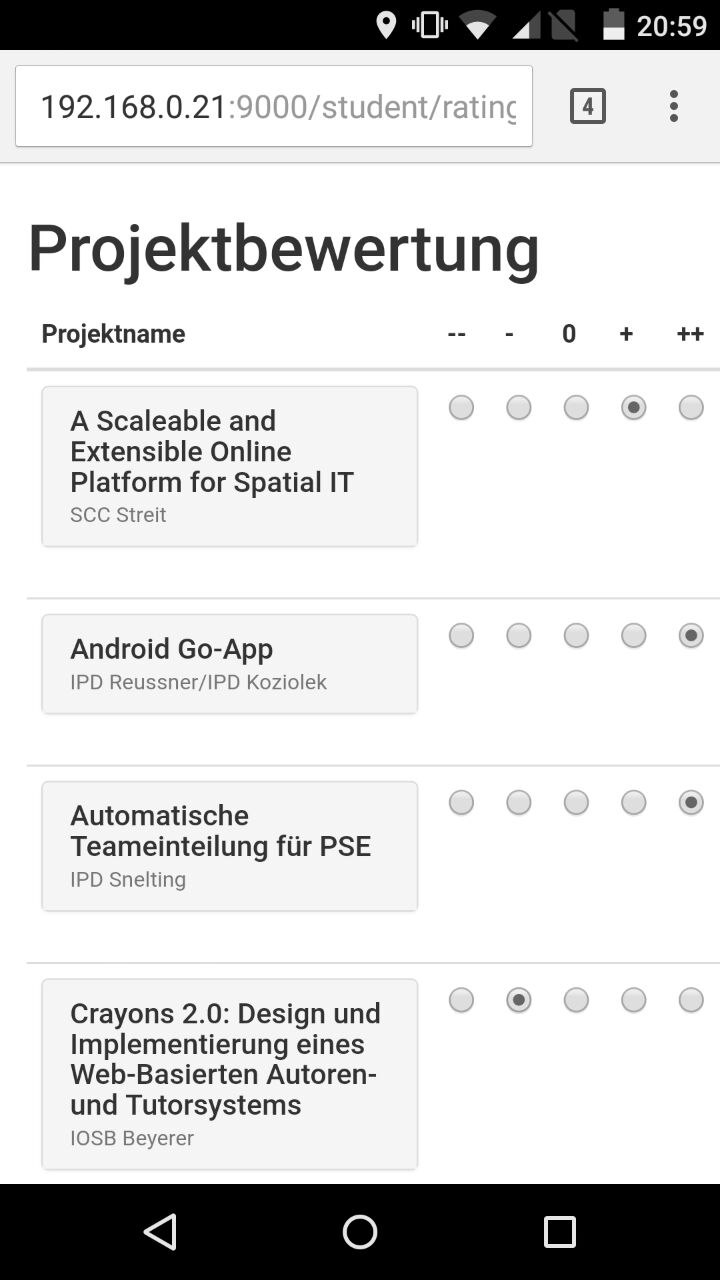
\includegraphics[height=0.7\paperheight]{bilder/androidScreenshot.png} &
	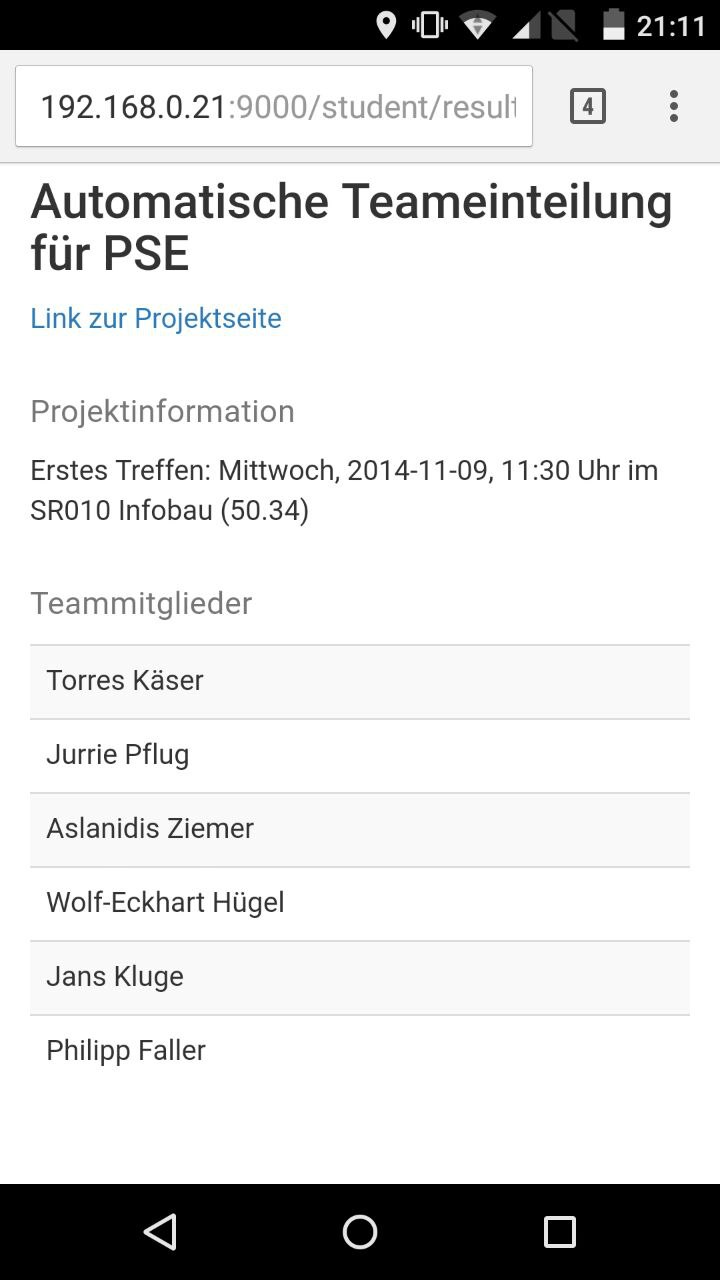
\includegraphics[height=0.7\paperheight]{bilder/android2Screenshot.png}	\\
	\end{tabular}
}
	}

\end{frame}

\subsection{Was würden wir anders machen?}
\begin{frame}{Was würden wir anders machen?}
	\begin{itemize}
		\item Besser über potentiell verwendete Bibliotheken informieren
	\end{itemize}
	
\end{frame}

\section{Live-Demo}
\begin{frame}
 \begin{center}
  \Huge Live-Demo
 \end{center}
\end{frame}

\end{document}
